\vspace{-0.5cm}
The Immelmann turn, named after German World War I flying ace Max Immelmann, is an an  aerobatic maneuver that results in level-flight of the aircraft in the opposite direction and higher altitude.

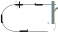
\includegraphics[width=\linewidth]{figures/immelmann-overview}
\captionof{figure}{Immelmann turn overview}
\label{fig:immelmann-overview}
\vspace*{0.5cm}

The aircraft initiates this maneuver in straight levelled flight, and describes an upwards semicircle contained in its symmetry plane. This increases the flight altitude while changing the trajectory's to the original's opposite direction and leaves the plane turned upside down. It then rolls while still flying in a straigth line, and returns to the initial condition of levelled flight.\\

This maneuver can be performed for various velocities and radius, but there are some dependencies and limitiations to be taken into account, such as the maximum deflections or forces the control surfaces can provide or support, respectively. 

The higher the velocity is, the bigger the radius - this is, the greater the increase of altitude - given that the wing's flaps cannot deflect enough nor can support as much force to reduce the radius as to the same menauver for a lower velocity.

Note that the centripetal force follows:
\[
	F=\frac{mV^2}{R}
\]
Where \textit{m}, \textit{V} and \textit{R} are the aircraft's mass (in kg), velocity (in m/s) and radius (in m) respectively. \\

The only angles affected are gamma $\gamma$ and mu $\mu$ if performed flawlessly. The former is the angle formed between the \textit{x} axis of the horizontal set and the \textit{x} axis of the wind set, while the latter is the one formed between the \textit{y} axis of the same sets. Note that for the whole maneuver the body set remains consistent with the wind set.\\
Figure \ref{fig:paramEvolution} shows how these change in the different phases of the Immelmann turn\\

	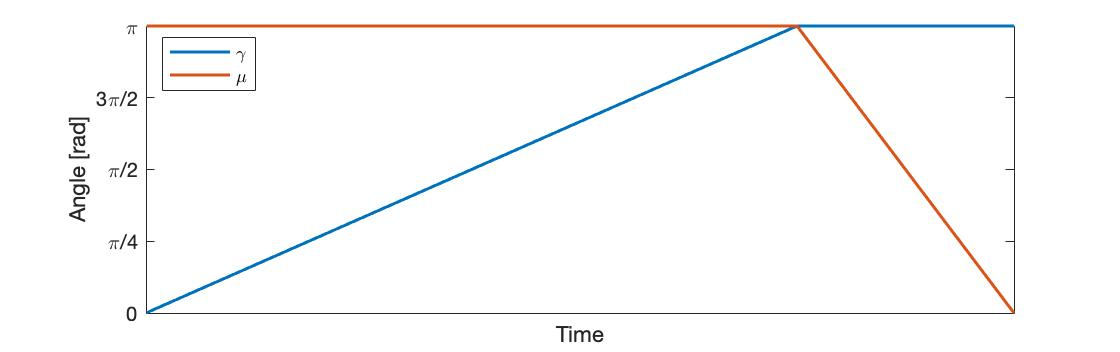
\includegraphics[width=\linewidth]{../matlab/paramEvolution.jpg}
	\captionof{figure}{Angles evolution over time}
	\label{fig:paramEvolution}
	\vspace{0.5cm}

Note that for $\gamma$ the evolution is perfectly defined, as the increment of said angle needs to be positive in order to increase the flight altitude. Conversely, for $\mu$ the pilot could choose to rotate in the opposite direction thus changing $\mu$ from 0 to $-\pi$ instead - note that $\pi$ and $-\pi$ are equivalent -, and the result would be virtually the same.\\
Furthermore, in order to describe a perfect semicircle the angular speed $\dot{\gamma}$ needs to remain constant. This results in the necessary condition of gamma's evolution to be a straight slope. For $\mu$, however, the pilot could also perform the roll at non-constant rotating speed without this having an impact on the maneuver performance. This would be reflected as a curve on mu's temporal evolution, instead of a straight line.

